\documentclass[11pt]{IEEEtran}

\usepackage{cite}
\usepackage{graphicx}
\graphicspath{{img/}}
\usepackage{hyperref}
\usepackage{tikz}
\usepackage{caption}
\usepackage{subcaption}
\usepackage[linesnumbered,lined,boxed,commentsnumbered]{algorithm2e}
\makeatletter
\newcommand{\removelatexerror}{\let\@latex@error\@gobble}
\makeatother


\begin{document}

% Subject : Symbolic executions technique for finding bugs %
\title{A Survey of\\Symbolic Executions Techniques} % NB: I removed the "for finding bugs" because "bug" is not well-defined and we can clearly state in the introduction why we use symbolic execution.
\author{Hallet Adrien, Sens Loan}
\date{\today}
\maketitle

  \section*{Abstract}
    % Describe paper's goals and content

  \section{Introduction}
    \subsection{A definition}
      % I tried to explain what is symbolic execution in simple concepts of software engineering
      The first occurences of symbolic execution described the then-new method as a middle ground~\cite{newapproach} between the two most-used method of its time: \emph{program testing} and \emph{program provign}.
      Nowadays, symbolic execution is both described as (part of) the core of many modern techniques to software testing\cite{chopper:icse18} and an effective way to create tests suites with extensive coverage.\cite{threedecadeslater}
    \subsection{The concept}
      The idea behind symbolic execution is to test an algorithm with \emph{symbolic values} rather than concrete values. So instead of using unit testing where a variable is set to a (usually random) value, the symbolic execution maintains a formula that contains all the possible values for the code to reach a particular point in the program. This formula is updated every time the program reaches a branching point. In figure~\ref{fig:symbolicsimple}, we show an example from~\cite{visserWillemCorina} of a symbolic execution. Observe how it produces constraints over the variables to explore the algorithm's branching tree.
      \begin{figure}
%      \subcaptionbox{Pseudo-code swapping 2 variable values and produce some errors}[.18\textwidth]{
%      	\removelatexerror
%      	\begin{algorithm}[H]
%      	 \scriptsize
%	    	\SetKwFunction{Ffoo}{foo}
%	    	\SetKwProg{Fn}{Function}{:}{}
%			    \Fn{\Ffoo{int x, int y}}{
%		    	\If{x $>$ y} {
%		    		x = x + y\;
%		    		y = x - y\;
%		    		x = x - y\;
%					\If {x $>$ y} {
%						ERROR1\;
%					}
%					\If {x $>$ 2} {
%						ERROR2\;
%					}
%		    	}
%		    	\KwRet SUCCESS\;
%	    	}
%	
%		\end{algorithm}
%      }
%      	\subcaptionbox{Corresponding symbolic execution tree}[.3\textwidth]{%    
%      	\tikzset{
%		  treenode/.style = {shape=rectangle, rounded corners,
%		                     draw, align=center
%		                     },
%		  unfeasible/.style = {treenode},%, bottom color=gray!30},
%		  error/.style      = {treenode},%, bottom color=red!30},
%		  sucess/.style     = {treenode},%, bottom color=lime!30},
%		  basic/.style      = {treenode},%, bottom color=blue!20},
%		  myLabel/.style = {draw=black, shape=rectangle},
%		  branchLabel/.style = {draw=none},
%		}
%
%		\begin{tikzpicture}[
%			scale = 0.6,
%			sibling distance = 150,
%			level distance = 55,
%		  	every node/.style = 
%		  	{
%		  		scale = 0.6,
%		  		shape=rectangle, 
%			    	draw, align=center,
%			    	top color=white,
%		    	}
%		    ]
%		\node[basic,label={[myLabel]left:0}] {$x:\lambda_1, y:\lambda_2$\\PC : $\langle \rangle$} 
%			child {node[basic, label={[myLabel]left:1}] {$x:\lambda_1, y:\lambda_2$\\PC : $\langle \lambda_1 > \lambda_2 \rangle$} 
%				child {node[basic,label={[myLabel]left:3}] {$x:\lambda_1 + \lambda_2 , y:\lambda_2$\\PC : $\langle \lambda_1 > \lambda_2 \rangle$}
%				{
%					child {node[basic, label={[myLabel]left:4}] {$x:\lambda_1 + \lambda_2 , y:\lambda_1$\\PC : $\langle \lambda_1 > \lambda_2 \rangle$} 
%						child {node [basic, label={[myLabel]left:5}]{$x:\lambda_2 , y:\lambda_1$\\PC : $\langle \lambda_1 > \lambda_2 \rangle$} 
%							child {node[unfeasible, label={[myLabel]6}] {$x:\lambda_2 , y:\lambda_1$\\PC : $\langle \lambda_1 > \lambda_2, \lambda_2 > \lambda_1 \rangle$\\ FALSE}
%								edge from parent node[branchLabel] {6}
%							}
%							child {node[basic, label={[myLabel]7}] {$x:\lambda_2 , y:\lambda_1$\\PC : $\langle \lambda_1 > \lambda_2, \lambda_2 \leq \lambda_1 \rangle$}
%								child {node[error, label={[myLabel]8}] {$x:\lambda_2 , y:\lambda_1$\\PC : $\langle \lambda_1 > \lambda_2, \lambda_2 > 2 \rangle$\\ERROR2}
%									edge from parent node[branchLabel] {8}
%								}
%								child {node[sucess, label={[myLabel]9}] {$x:\lambda_2 , y:\lambda_1$\\PC : $\langle \lambda_1 > \lambda_2, \lambda_2 \leq 2 \rangle$\\SUCCESS}
%										edge from parent node[branchLabel] {8}
%								}
%								edge from parent node[branchLabel] {6}
%							}
%							edge from parent node[branchLabel] {5}
%						}
%						edge from parent node[branchLabel] {4}
%					}
%					edge from parent node[branchLabel] {3}
%				}
%			}
%				edge from parent node[branchLabel] {2}
%			}
%			child {node[sucess,label={[myLabel]2}] {$x:\lambda_1, y:\lambda_2$\\PC : $\langle \lambda_1 \leq \lambda_2 \rangle$\\SUCCESS}
%			edge from parent node[branchLabel] {2}
%			}
%		;
%		\end{tikzpicture}
%		}
		\centering
        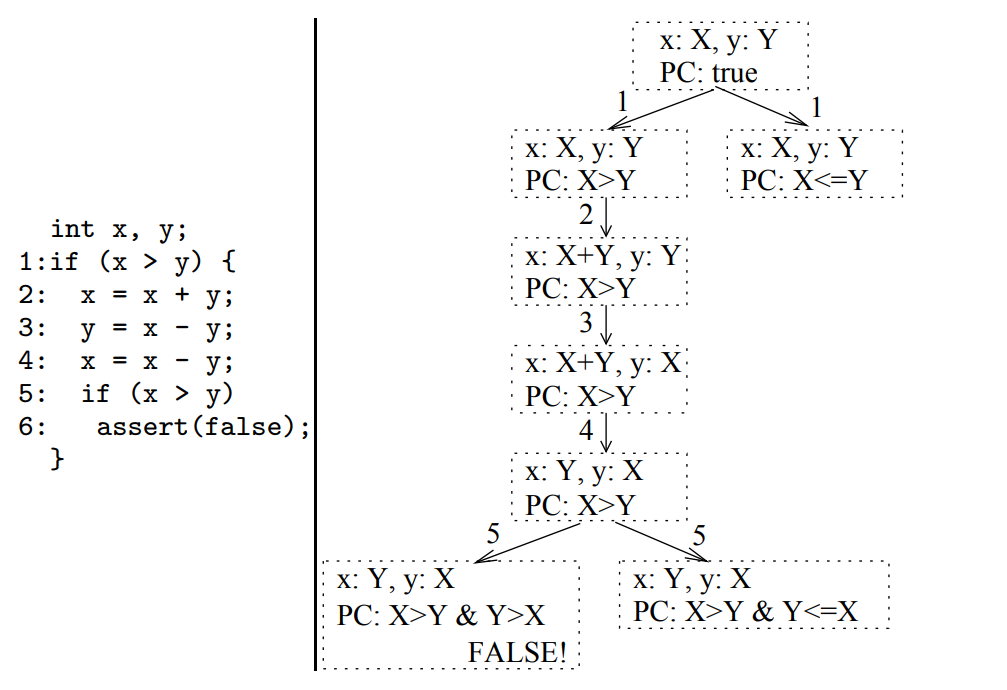
\includegraphics[width=0.5\textwidth]{symbolicsimple}
        \caption{Swapping two integers and its symbolic execution tree}
        \label{fig:symbolicsimple}
      \end{figure}
    % What is symbolic execution and why do we do this survey
  \section{History}
    We find the first papers on symbolic execution around 1975~\cite{newapproach}. Early methods proposed simple structures to hold conditions with a SAT-solver, the support of simple data types and were focused on algorithm testing (instead of large programs). While papers continue to grow on the subject, it really is around 2005 that symbolic execution gets wind in its sails with more and more frameworks and tools for software verification. The last ten years have seen more papers on the subject\footnote{Data from Google Scholar} (around 200.000) than the three decades following its introduction (half that much). Among the supporters of the method, we can identify two clear research poles, China~\cite{Hardware, memorytablemodel, CHEN2018118} and the United States of America, with an heavy participation of Microsoft~\cite{bouncer-securing-software-by-blocking-bad-input} which was pooling heavy resources in software and OS reliability, and the NASA~\cite{neurosymbolicexecution, DirectedIncrementalSymExe, visserWillemCorina}.

  \section{Method}
    % Begin with anything general to say (if any) then detail methods, could also be useful to compare them (if possible) and/or to say when/why a particular method is being used instead of another.
    \subsection{Useful concepts}
      Algorithms can be modeled as graphs where nodes are basic blocks (\emph{i.e.: a part, one or multiple instructions with a single entry and exit point}) and edges are the branches (issued from conditional statements). Def-use pairs use the same concept, although they base their graph on the \emph{definition} and \emph{usage} of a variable. With the \emph{branches} and \emph{def-use pairs}, we can model an algorithm's behavior to follow the values of its variables and determine the \emph{execution path}.
    \subsection{Basis}
      \label{sub:basis}
      Symbolic execution works on those concepts by updating an internal list of symbols. The execution generates a new symbol for each introduced variable in an algorithm\cite{newapproach}. The symbolic execution runs over the algorithm's statements and builds the symbolic values when it encounters a branching point. The symbolically executed algorithm creates a \emph{state}\cite{visserWillemCorina} containing the symbolics values, a counter identifying the next line to be executed and a \emph{path condition}. This path condition is a simple boolean formula over the symbols, it creates a constraint for the algorithm to reach the current state of the program (this also allows to check for unreachable paths in programs~\cite{InfeasiblePathsEliminationWithSymbolicExecTechniques}). The path condition allows to recreate the execution up to its state. The states are stored in a \emph{symbolic execution tree} with the states as nodes and the transitions as edges (see figure~\ref{fig:symbolicsimple}).
    \subsection{Problems}
      \label{sec:problems}
      \subsubsection{State-Space Explosion}
        \label{subsec:state-space-explosion}
        Symbolic Execution cannot be that perfect and hosts its bundle of problems that reduce either the confidence in or the performances of the concept. We have seen symbolic execution tree in~\ref{sub:basis}. Small algorithms can use such methods but actual programs need to be tested in \emph{integration}. In large environments, the tree's branching factor will produce too many nodes (\emph{state-space explosion}) for the performances to stay relevant, sometimes creating infinite loops in the graph~\cite{forwardSymbolicExecution}. Reducing the state space or pruning them is not enough. To improve the performances, we can depth-first-search the graph but it does not prevent infinite loops until we add a max depth (as KLEE or EXE do, see sections~\ref{subsec:exe},~\ref{subsec:klee}).
        Pruning heuristics (\emph{e.g.:def-use pairs distance}) can be used to reduce the tree's branching factor, we may randomly select a path (emph{i.e: the path condition}), weighting the shallowest nodes to avoid dead-loops. The random technique is exploited by a lot of \emph{fuzzing techniques}~\cite{CHEN2018118} which uses the injection of random values to detect program's faults. Another solution lies in the \emph{concolic execution} (see~\ref{subsec:concolicExecution}). Very recently (july 2018), a team of researchers~\cite{neurosymbolicexecution} managed to successfully test programs that were previously untested due to complex memory usage leading to complex explosion. They used a new approach with neural networks to solve the constraints within the states.

      \subsubsection{Modeling the memory}
        Another technical difficulty lies in the \emph{memory model}. As said before, a symbol $\alpha$ represents a variable \texttt{a} with a value. In the programming world, it means there is a pointer \texttt{a*} that stores the address to an allocated memory block. The initial approach~\cite{newapproach} proposed a \emph{fully symbolic memory}. The symbols are stored in plain states holding their path condition with either a duplication of the states depending on their memory status called \emph{state forking} where every possible execution is forked from the main branch (\emph{e.g.: accessing an array of size 10 with a variable $i$ that depends on the context will fork 10 states from the main memory state, each one with $i$ from 0 to 9}). Fully symbolic memory is therfore slowed by an increased \emph{state-space explosion}. To reduce memory usage, some tools may represent an artificial memory space~\cite{5635129}, which reduces the size of the general space by allowing more memory to each path condition, although doing so will void some execution paths, leaving potential bugs out of the symbolic execution. An italian approach~\cite{memorymodelpointers} proposes the use of a \emph{symbolic} adress which holds the condition to which address the variable points to, which drastically reduces the amount of memory states.

        Instead of fully modeling the memory, there also is the \emph{abstract symbol table}~\cite{memorytablemodel} which records tuples [variable, address, symbolic value]. This method has the advantage of supporting complex data types (some fully memory models cannot express structures) and memory aliasing (instead of creating a new variable copied from another in older methods).
  \section{Variants}
    % I split the section because it was too heavy for my liking and I think we can better state the base and what challenges it produces, then look at how we can solve them with variants. It also allows the reader to just skip the variants in the future if he just wants to know about the method.
    \subsection{Concolic execution}
    \label{subsec:concolicExecution}
    	\emph{Concolic}, portmanteau from \emph{concrete} and \emph{symbolic}, is a testing method in which we mix symbolic executions alongside concrete ones. Using both concrete and symbolic values is a widely used technique that many contemporary tools use because of its ability to speed up the execution while reducing the used memory.\\

    	\subsubsection*{Concolic execution approaches}
    		This technique concept was first introduced in 2005 \cite{godefroid2005dart} (more details on section \ref{subsec:DART}). % The name used wasn't "Concolic" yet but the concept idea was the same
    	  Since then the idea was further extended and combined with other testing techniques.\\

  		\subsubsection{Dynamic Symbolic Execution}
  		\label{subsec:dynamicSymbolicExec}
  			\emph{Dynamic Symbolic Execution} (DSE) also kwown as \emph{dynamic test generation} \cite{godefroid2005dart} is a popular approach of concolic execution. Its main concept is to drive the symbolic execution by the concrete execution.\\

  			For this method, we will first need to add a new store, a memory structure, in order to save the concrete execution information.\\
  			The first step involves choosing an arbitrary value as input for our parameters. Then it executes the program concretely and symbolically concurrently, updating both the stores and the path constraints. When the concrete execution is directed on a certain branch, the symbolic execution follows it and the constraint is appended the the set of path constraints.\\
  			In order to explore different paths, we generate new control flows by negating one or more constraints. We can repeat this process as many time as we want to achieve the desired coverage.\\

  			Note that different strategies exist on the choice of the branch to negate, this choice depends on the used tool.\\

  		\subsubsection*{Downside : Imperfect symbolic execution}
  			\begin{itemize} % description layout act strangely here
  				\item \emph{False Negative} : Missed path. For example, when another function from the one currently tested has no symbolic tracking but needs the result to further explore the branch.
  				\item \emph{Path Divergence} : In some situations the symbolic engine can produce false positive because of the \emph{isolation problem}(see section~\ref{subsec:exe}). The tool then returns an input that can provoke an error in the program, only that said input cannot exist in the context. For example, the absolute value function could be called in a program. The same program would later use the value and the symbolic engine will signal an error for a negative value. Only a negative value cannot exist because of the absolute value, but the path condition has not been updated because the solver did not know how the external call changed the constraints. \\ % J'espère que c'est plus clair.
  				According to \cite{Godefroid2008AutomatedWF} they calculated a divergence rates of over 60 \%
  			\end{itemize}

    	\subsubsection{Selective Symbolic Execution}
    	\label{subsec:selectiveSymbolicExec}
    		This approach is based on the observation that often only some families of paths are meaningful\cite{chipounov2012s2e}. We focus the exploration on some designated interesting components of the software while not caring about the others. It offers an illusion of symbolically executing a full software, when in reality it only executes a partial symbolic execution on the tested components.\\

    		The selective symbolic execution switches back and forth between symbolic and concrete execution, depending on the current component's relevance. When it is symbolic, the tree may expand in width (higher branching factor) and depth, on the other hand, in a concrete execution it only grows in depth as only one branch is created (see Figure \ref{fig:selectiveSymbolicExample} ).
    		\begin{figure}
    			\centering
    			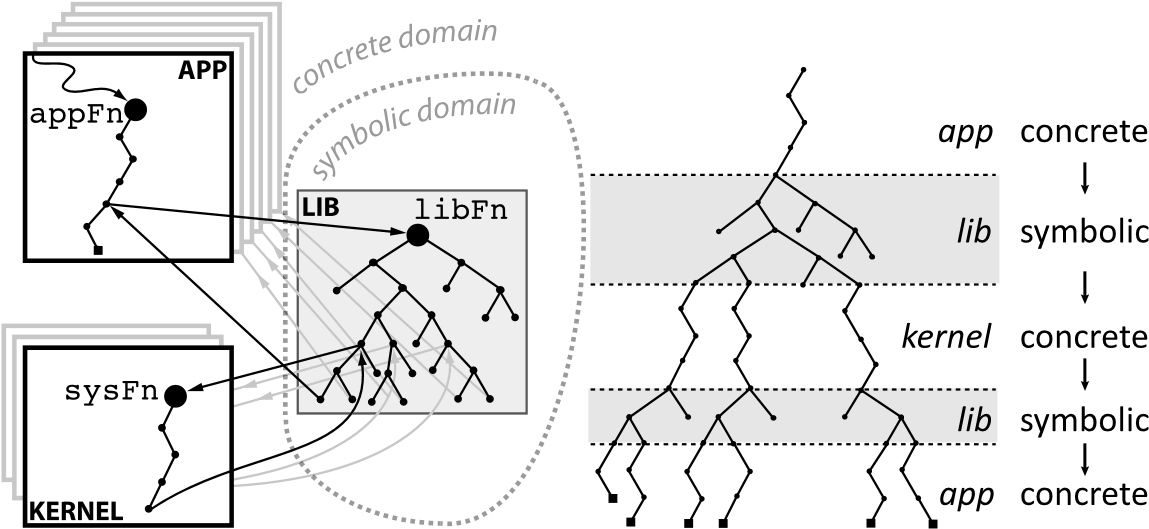
\includegraphics[scale=0.9]{selectiveSymbolicExecExample.png}
    			\label{fig:selectiveSymbolicExample}
    			\caption{Multipath/single-path execution: three different modules (left) and the resulting execution tree (right). Gray shaded areas highlight symbolic execution, while the white are concrete executions. More details in section \ref{subsec:S2EExample}}
    		\end{figure}

  \section{Tools and languages}
  %TODO : autre outils potentiels : SAGE
  	Many tools exist for symbolic execution, \href{https://en.wikipedia.org/wiki/Symbolic_execution\#Tools}{Wikipedia} mentions 22 of them. Another \href{https://github.com/ksluckow/awesome-symbolic-execution\#tools}{source} claiming to \emph{curate a list of awesome symbolic execution resources including tools} mentions 35 different tools spread over 10 different languages.\\

    % Let DART be first as it is the first used tool to use concolic
    \subsection{\emph{DART} : Directed Automated Random Testing}
    \label{subsec:DART}
    	\emph{DART} is presented as a tool for automatically testing software using concolic testing method. It was introduced in 2005, placing it as the first tool to be created using concolic techniques, and more specifically dynamic symbolic execution techniques (see section~\ref{subsec:dynamicSymbolicExec}). \\

    	\subsubsection{Methodology}
	    	\emph{DART} combines three main techniques~\cite{godefroid2005dart} in order to automate the process of testing for a particular software:
	    	\begin{enumerate}
	    		\item \emph{Automatic extraction of program interface}: Extract the interface of a program, including its external environment by using static source-code parsing.
	    		\item \emph{Automatic test generation}: Generate a test driver for this interface. It will perform random testing simulation using the most common environment the program may execute in.
	    		%Automatic generation of a test driver for this interface that performs random testing to simulate the most general environment the program can operate in
	    		\item \emph{Dynamic analysis}: Perform a dynamic analysis on how the program behaves under random testing and automatic generation of new test inputs to drive systemically the execution along different program paths.
	    	\end{enumerate}

			\emph{DART} chooses the \emph{depth-first search} strategy whenever it has to negate a branch.

	    \subsubsection{Example}
		    Let consider the following program :

		    \begin{algorithm}
		    	\SetKwFunction{Ffoo}{foo}
		    	\SetKwProg{Fn}{Function}{:}{}

		    	\Fn{\Ffoo{int x, int y}}{
			    	\If{x != y} {
						\If {2 * x == x + 10} {
							ERROR\;
						}
			    	}
			    	\KwRet SUCCESS\;
		    	}

		    \end{algorithm}

	    	This function is defective as it may lead to an error statement for some value of $x$ and $y$.\\
	    	\emph{DART} start by guessing values for both $x$ and $y$ for instance $269167349$ and $889801541$. With these values the function return  successfully, during the execution two predicates were formed created by the \texttt{if} statements, in our case the final path constraint is: $\langle x_0 \neq y_0, 2 \times x_0 \neq x_0 + 10 \rangle$ with $x_0$ and $y_0$ being \emph{symbolic variables}.\\
	    	While we maintain these predicates, all paths will lead to the same termination. So in order to force the program through a potential different outcome we change one of the predicate and look at the result. If we negate the last predicate we have the following path constraint: $\langle x_0 \neq y_0, 2 \times x_0 = x_0 + 10 \rangle$ in which $x_0=10$ and $y_0=889801541$ are solutions. Using these values as inputs, the program end up in the \texttt{ERROR} state, as desired.

	    \subsubsection{Key strength/originality}
	    	One of the main strengths of DART is that, on any compilable program, testing can be performed completely automatically. There is no need to write any additional harness code or test driver.\\
	    	During testing, DART detects standard errors such as program crash, assertion violation, and non-termination.\\
	    	Because it is based on precised dynamic analysis, DART provides an interesting alternative to static analyzers. It is expected to be very good at the detection of some kind of bugs\footnote{Especially interprocedural bugs and bugs that happen through library functions use} compared to a dynamic analyzers.\\
	    	Any errors found by DART during the execution is sure to be sound.\\

	    	But DART has its own limitations, particularly the limited effectiveness of dynamic test generation to improve over random testing and the computational cost of running tests.

	\subsection{Cute \& jCUTE}
		\emph{CUTE} and \emph{jCUTE} are automated concolic testing tools, CUTE stands for Concolic Unit Testing Engine\cite{sen2006cute}. The first one is for \emph{C} programs while the second one target \emph{Java} ones.\\

		Both tools consist of two main modules :
		\begin{itemize}
			\item \emph{Instrumentation}\footnote{more precisely it uses \emph{CIL} and \emph{SOOT} compiler frameworks}: to add some code in the program under test so that the program calls the library.
			\item \emph{Library}: to perform symbolic execution, solve constraints and control thread schedule.
		\end{itemize}

		As of today, \emph{CUTE} is obsolete and has been replaced by \emph{CREST}~\cite{CuteWebSite}. The last commit on the \href{https://github.com/jburnim/crest}{official repository of the project} dating back to 2017. \\
		\emph{jCUTE} is the first concolic execution engine for \emph{java}~\cite{jDart} designed and implemented around 2006. It is no longer maintained, the last commit on the \href{https://github.com/osl/jcute}{official repository of the project} dating back to 2013.

	\subsection{JDART}
		\emph{JDART} describes itself as a dynamic symbolic analysis framework for \emph{Java} \cite{jDart}.\\
		The main goal of the tool is to build a dynamic symbolic analysis tool that can be used at industrial scale complex softwares. Another important aspect was the main design guideline; they wished it to be modular and extensible.\\

		%TODO [Loan] : Si nécessaire, parler plus en profondeur des features de JDART "As mentioned, the key distinguishing feature of JDart is its modular architecture.The two main components of JDart are the Executor and the Explorer ."

		Looking at the \href{https://github.com/psycopaths/jdart}{repository of the project}, it started around 2015. But it seems that it stagnates since 2017 based on the code activity.
		% JDART parle de JCUTE dans la section 4 : "Several symbolic execution tools specifically target Java Bytecode programs. A number of them implement dynamic symbolic execution via Java Bytecode instrumentation. JCute [27], the first concolic execution engine for Java, uses Soot [30] for instrumentation, and uses lp_solve as a constraint solver. JCute is no longer maintained."

		%TODO : relation entre JDART et JPF : "Currently, JDart uses the software model checker Java PathFinder (JPF) for the execution of Java Bytecode programs." Mais on ne parle pas de JPF encore, donc ça ne serai pas pertinent

  \subsection{EXE}
    \label{subsec:exe}
    Section~\ref{subsec:state-space-explosion} stated the memory problem. \textbf{EXE} is a tool (focused on C) that aims to reduce that with the use of concolic execution within the states, allowing to partially store the states and using the path condition to recreate the output if needed. The tool bases itself over the principle of \emph{EGT - Execution Generated Testing}~\cite{exe}, which is basically the classic approach to symbolic execution. The tool uses a constraint solver working on the path condition to prune the tested algorithm's branches (simply deleting unsatisfiable constraints, branches that cannot logically exist can be generated due to the symbolic value, this pruning removes them), then to solve the constraint to generate a set of test value. The tool also uses models to check code coverage, which is only optional.

    Although good for its time, EXE still suffers from the same problems and a new one; \emph{isolation}. The tool is isolated from the environment and any kind of interaction ruined the double execution of symbolic and concrete data. Interacting with a network, input, ... would result in the loss of the symbolic execution or would require a full model of the world to interact with (which ranges from difficult to impossible). Furthermore, the need for a model for sufficient coverage requires a realistic and complete model. Functions which return the same value for different outputs (\emph{e.g.: in Java, if you compare an object to another}) or worse; different values for the same input, would result in models that would not quite work with the tool. On top of that, the tool works assuming it has a good SAT-solver (and as we know, 3-SAT is np-complete) and available memory.

  \subsection{KLEE}
    \label{subsec:klee}
    This tool~\cite{klee} is a complete rework of EXE, also focused on C, by the same authors three years later (2008). While the basis were the same, KLEE managed to largely improve the execution time and space by keeping its advantages (\emph{exact memory representation}, constraint solving, high code coverage). To reduce the space bottleneck, KLEE stores the states concurrently, sharing them, allowing larger sets of states to be used by the same execution. It is important to note that KLEE does not mindlessly check each instruction. Sets of dangerous operations which can lead to failures rather than wrong outputs are determined. In the C-language context, it means memory accesses and allocation. Each time the solver reaches one of those dangerous operations in an algorithm, KLEE tries all the values allowed by the current path condition and returns all the inputs leading to faulty results.

    KLEE is arguably one of the most advanced symbolic execution frameworks up to this day. Its new architecture~\cite{klee}, inherited from the EXE's experience, reduces usage complexity, time and space. To reduce \textbf{memory} usage, KLEE does not use a OS-generated program state as EXE did, but instead maps pages tables to a virtual heap to share memory, similar to a forking process accessing shared memory. It is called \emph{compact internal state representation}, increasing the concurrent state amount without decreasing the memory representation quality. To reduce \textbf{time} (in relation to other symbolic execution tools), KLEE introduces many \emph{sat-solving optimisations}. As satisfiability is a NP-complete problem and KLEE generates many of constraints that have to be solved (either to reduce a path condition form or to find a faulty input from the path condition), we can expect high computation times. The tool is able to reduce this execution time up to 15 faster than without optimisations. We can observe~\emph{klee} :
    \begin{itemize}
      \item \emph{Expression simplification}: maintain the most simple path condition everytime a constraint is added to reduce further computation time. For example, if a first branch requires a positive number and a second condition along this path requires an integer between 10 and 20, we can drop the first condition.
      \item \emph{Implied value concretization}: we have seen that both EXE and KLEE sometimes use concrete value because they are cheaper. If during an execution the condition of a variable is an equation, KLEE solves the equation to store the concrete(s) value(s) of the variable instead of a path condition.
      \item \emph{Constraint independance}: inherited from EXE, this optimisatin stores the constraints in groups sorted by the accessed variables. Constraints that do not access the same variable have no need to be checked simultaneously because they do not overlap.
      \item \emph{Counter-exemple cache}: is a cache of queries to eliminate both redundant queries (slightly similar to expression simplification) and unsolvable queries via a map of the constraints. We could therefore eliminate ${x < 0, x > 0}$ as soon as the constraint is introduced.
    \end{itemize}
    The tool also speeds execution up with the use of both complex heuristics on the paths and path conditions (they also use random path exploration). As many of the symbolic execution tools, KLEE has been open source since 2009~\footnote{https://github.com/klee/klee} and is still active today. On the negative side, we can note that KLEE does not support multithreaded algorithms, and has trouble with complex memory objects (especially those varying in size and symbolic floating points).

	\subsection{S$^2$E}
    \label{subsec:S2E}
    	S$^2$E is a platform for writing tools that analyze the behavior and properties of software system. It comes as a modular library that gives virtual machines symbolic execution and program analysis capabilities.\cite{S2EWebSite} It uses selective symbolic execution concolic execution (see section  \ref{subsec:selectiveSymbolicExec}).\\

		The platform is related to the previously mentioned KLEE tool (see section \ref{subsec:klee} ) as S$^2$E is built upon its engine and the QEMU virtual machine emulator.
    	The platform was launched in 2011 and is still update until now according to last commits on the \href{https://github.com/S2E}{project repository}.

    	\subsubsection{Methodology}
    		S$^2$E switches dynamically between symbolic and concrete execution. This transition is not trivial and must be treated separately.\\
    		Let \texttt{A} and \texttt{B} be functions such as \texttt{A} calls \texttt{B}.\\
    		\subsubsection*{From concrete to symbolic and back}
    			\texttt{A} calls \texttt{B} with concrete arguments (because \texttt{A} is a component that is not symbolically relevant) as we are still in a concrete execution. However \texttt{B} is symbolic, therefore it modifies the arguments sent by \texttt{A} to make them symbolic. For instance \texttt{B(10)} becomes \texttt{B($\lambda$)}. In can additionally be set to some constraints, for example \texttt{B($\lambda < 15$)}.\\
    			After the transition occurs, S$^2$E symbolically executes \texttt{B}, concurrently using the symbolic argument(s) and the concrete argument(s).\\
    			Once the exploration of \texttt{B} is over, S$^2$E returns the concrete execution's final value to \texttt{A}.\\
    			This way, the execution of \texttt{A} is always consistent, meanwhile S$^2$E uses the extra symbolic path in its analyzer plugin to check for possible issues.

    		\subsubsection*{From symbolic to concrete and back}
    			\texttt{A} calls \texttt{B} with symbolic arguments (because \texttt{B} is a component that is not symbolically relevant) as we are still in a symbolic execution. However \texttt{B} is concrete, therefore it modifies the arguments sent by \texttt{A} to make them concrete while still maintaining path constraints. For instance if we have the path constraint  $\langle \lambda < 5 \rangle$, we can choose -20 or 3 as a concrete value but not 5 or 42.\\
    			After this choice, \texttt{B} execute concretely then return symbolically back to \texttt{A} which resume symbolically.\\
    			Note that S$^2$E actually employs \emph{lazy-concretization}: It converts the value of $\lambda$ from symbolic to concrete on-demand, only when the concrete execution is about to branch on a condition that depends on the value of $\lambda$. \\

    			It is important to mention that this transition may lead to the \emph{overconstraining} problem, which impact both the soundness and completeness of the tool. The problems that may arise can be :
    			\begin{itemize}
    				\item Exclusion of paths due to the concretization of the arguments.
    				\item Exclusion of paths indirectly due to the the constrained return value
and side effects.
    			\end{itemize}
    			%TODO : il y aurait une solution à ce problème en marquand les contraitnes comme "soft" ou quoi, à approfondir si on à le temps

    	\subsubsection{Example}
    	\label{subsec:S2EExample}
    		Let us use the figure \ref{fig:selectiveSymbolicExample} as a reference example, it describes an application \emph{app} using a library \emph{lib} on top of an OS \emph{kernel}. We are interested in testing the \emph{lib}, but not the \emph{app} nor the \emph{kernel}. Therefore only the \emph{lib} will be executed symbolically, the 2 others will be concrete.\\

    		\emph{app} call the function \emph{appFn} which itself calls a \emph{lib} function \emph{libFn}, which eventually invokes a system call \emph{sysFn}. After that \emph{sysFn} returns, \emph{libFn} does some extra execution and then eventually returns to \emph{appFn}. Once the execution crosses into the symbolic domain (gray shaded part) from the concrete domain (white part), the execution tree expands. After the execution returns again to the concrete domain, the execution tree no longer expands, it may still grow, but it does not add any new paths until the execution goes in the symbolic domain again. A path may terminate prematurely, for example in case of hitting a crash bug.



  \section{Conclusions}
    We hope that this survey has been a good introduction to the world of symbolic execution, both in the general context and the current tools that are still being developed since what we could call a rebirth of the field in 2005, thanks to the big companies previously cited (see History). It is also important to note that softwares are not the only ones being symbolically tested. While not discussed here, we can cite usage of symbolic execution in hardware~\cite{Hardware} and networks~\cite{220590}. Due to the limited size of this paper, we were not able to extensively look into techniques and complex mechanisms but we hope that we planted a seed of curiosity or interest in the subject. To wrap this survey up, we could insist on the emergence of more and more complex tools that, while still being slowed down by the almighty state-space explosion, gain in power each year. Symbolic Execution, for now, is still a program testing solution that is mainly used in academia or large companies that can afford it. Small and medium companies still prefer unit and integration testing that is easier and cheaper to setup and maintain. But this could change in the future.\hfill % fill the rest of the page

    % What can we get from this paper in general
    % Could be pertinent to talk about a kind of "to go further" which could contain adjacent fields of research
    % Could be pertinent to talk about the future of symbolic execution, if there is any new technique being developed, ...


\pagebreak
\bibliography{bibliography}{}
\bibliographystyle{plain}
\end{document}
